We provide a more detailed analysis of the stopping rule introduced in Section \ref{sec:stopping_rule}.

\subsection{Anytime-valid $e$-processes}
\label{subsec_app:mmc_recursive}

Recall the predictable, recursive counts
\[
A_{n-1}:=\widehat c_{\,n-1},\quad B_{n-1}:=j^\star_{\,n-1},\qquad
\begin{aligned}
&s_n=s_{n-1}+\mathbf 1\{X_n=A_{n-1}\},\\
&f_n=f_{n-1}+\mathbf 1\{X_n=B_{n-1}\},\\
&o_n=o_{n-1}+\mathbf 1\{X_n\notin\{A_{n-1},B_{n-1}\}\},
\end{aligned}
\]
and the effective sizes \(M_n:=s_n+f_n\) (A vs B) and \(T_n:=s_n+o_n\) (A vs others).


Let $(\pi^{\mathrm{run}}_n)_{n\ge1}$ and $(\pi^{\mathrm{oth}}_n)_{n\ge1}$ be  {predictable} priors (each $\pi_n$ is $\mathcal F_{n-1}$-measurable) 
supported on $(1/2,1]$.
Define the two mixture $e$-processes recursively (with optional skipping) by
\begin{align*}
e^{\mathrm{run}}_n
&=\begin{cases}
e^{\mathrm{run}}_{n-1}\cdot 2\!\displaystyle\int \theta\,\pi^{\mathrm{run}}_n(d\theta), & X_n = A_{n-1},\\[1mm]
e^{\mathrm{run}}_{n-1}\cdot 2\!\displaystyle\int (1-\theta)\,\pi^{\mathrm{run}}_n(d\theta), & X_n = B_{n-1},\\[1mm]
e^{\mathrm{run}}_{n-1}, & \text{otherwise,}
\end{cases}\\[2mm]
e^{\mathrm{oth}}_n
&=\begin{cases}
e^{\mathrm{oth}}_{n-1}\cdot 2\!\displaystyle\int \lambda\,\pi^{\mathrm{oth}}_n(d\lambda), & X_n = A_{n-1},\\[1mm]
e^{\mathrm{oth}}_{n-1}\cdot 2\!\displaystyle\int (1-\lambda)\,\pi^{\mathrm{oth}}_n(d\lambda), & X_n \notin \{A_{n-1},B_{n-1}\},\\[1mm]
e^{\mathrm{oth}}_{n-1}, & \text{if } X_n = B_{n-1},
\end{cases}
\end{align*}
with $e^{\mathrm{run}}_0=e^{\mathrm{oth}}_0=1$.
By aggregating the per-round factors, we have the equivalent expression (\ref{eq:e_process_A_vs_B}) and (\ref{eq:e_process_A_vs_OTHERS}).


Before proving Theorem \ref{thm:mmc_eprocess_recursive}, we introduce the following auxiliary lemma.

\begin{lemma}[One-step mixture bound]\label{lem:onestep_recursive}
Let $\pi$ be any probability measure on $(1/2,1]$ and define $m:=\int u\,\pi(du)\in(1/2,1]$.
If $Y\sim\mathrm{Ber}(\vartheta)$ then
\[
\mathbb E\!\Big[\,2\!\int u^{Y}(1-u)^{1-Y}\,\pi(du)\,\Big] \;=\; 2\big(1-m+\vartheta(2m-1)\big),
\]
which is increasing in $\vartheta$ and $\le 1$ for all $\vartheta\le \tfrac12$, with equality at $\vartheta=\tfrac12$.
\end{lemma}

\begin{proof}
$\mathbb E[u^{Y}(1-u)^{1-Y}]=\vartheta u + (1-\vartheta)(1-u) = (1-u)+\vartheta(2u-1)$; integrating over $\pi$ yields the result.
\end{proof}

\begin{theorem}[Theorem \ref{thm:mmc_eprocess_recursive} restated]
Let $p_j=\mathbb P[X=j\mid pr]$. For the \emph{A vs B} test (leader vs runner-up), define
$\theta_n = \tfrac{p_{A_{n-1}}}{p_{A_{n-1}}+p_{B_{n-1}}}$ and the one-sided composite null
\[
H^{\mathrm{run}}_0:\quad \theta_n \le \tfrac12 \ \big(\text{equivalently $p_{A_{n-1}}\le p_{B_{n-1}}$}\big) \,\,\text{at every round $n$.}
\]
For the \emph{A vs others} test, define
$\lambda_n = \tfrac{p_{A_{n-1}}}{p_{A_{n-1}}+\sum_{j\notin\{A_{n-1},B_{n-1}\}}p_j} = \tfrac{p_{A_{n-1}}}{1-p_{B_{n-1}}}$
and the composite null
\[
H^{\mathrm{oth}}_0:\quad \lambda_n \le \tfrac12 \ \big(\text{equivalently $p_{A_{n-1}}\le \scriptstyle{\sum_{j\notin\{A_{n-1},B_{n-1}\}}}$$\, p_j$}\big) \,\,\text{at every round $n$.}
\]
Then $\{e^{\mathrm{run}}_n\}_{n\ge0}$ and $\{e^{\mathrm{oth}}_n\}_{n\ge0}$ defined in (\ref{eq:e_process_A_vs_B}), (\ref{eq:e_process_A_vs_OTHERS}) are non-negative test
\emph{supermartingales} w.r.t.\ $\{\mathcal F_n\}$, even with predictable, data-dependent priors and optional skipping.
Under the boundary (simple) nulls ($\theta_n\equiv\tfrac12$ or $\lambda_n\equiv\tfrac12$ on their informative rounds),
they are test \emph{martingales}. Consequently, by Ville’s inequality, for any stopping time,
\[
\sup_{\mathbb P\in H^{\mathrm{run}}_0}\ \mathbb P\Big(\sup_{n\ge0}e^{\mathrm{run}}_n\ge 1/\varepsilon\Big)\le\varepsilon,
\qquad
\sup_{\mathbb P\in H^{\mathrm{oth}}_0}\ \mathbb P\Big(\sup_{n\ge0}e^{\mathrm{oth}}_n\ge 1/\varepsilon\Big)\le\varepsilon.
\]
\end{theorem}

\begin{proof}
Fix $n\ge1$ and condition on $\mathcal F_{n-1}$, then $A_{n-1},B_{n-1}$ and the priors
$\pi^{\mathrm{run}}_n,\pi^{\mathrm{oth}}_n$ are deterministic. For the \emph{A vs B} process,
\[
\frac{e^{\mathrm{run}}_n}{e^{\mathrm{run}}_{n-1}}
=\begin{cases}
2\!\int \theta'\,\pi^{\mathrm{run}}_n(d\theta'), & X_n=A_{n-1},\\
2\!\int (1-\theta')\,\pi^{\mathrm{run}}_n(d\theta'), & X_n=B_{n-1},\\
1, & \text{otherwise.}
\end{cases}
\]
Write $q_n:=p_{A_{n-1}}+p_{B_{n-1}}$ and $\theta_n:=p_{A_{n-1}}/q_n$ (if $q_n=0$ the step is skipped a.s.).
Then, under $H^{\mathrm{run}}_0$ we have $\theta_n\le \tfrac12$ and
\[
\mathbb E\!\left[\frac{e^{\mathrm{run}}_n}{e^{\mathrm{run}}_{n-1}}\ \Big|\ \mathcal F_{n-1}\right]
= q\cdot \mathbb E\!\Big[\,2\!\int \theta'^{Y}(1-\theta')^{1-Y}\,\pi^{\mathrm{run}}_n(d\theta')\,\Big]
\;+\; (1-q)\cdot 1,
\]
where $Y\sim\mathrm{Ber}(\theta_n)$ on the informative event. By Lemma~\ref{lem:onestep_recursive},
the bracketed expectation is $\le 1$ for $\theta_n\le 1/2$, hence the whole conditional expectation is $\le 1$.
Thus $\{e^{\mathrm{run}}_n\}$ is a test supermartingale (and a martingale at $\theta_n=1/2$).

Similarly, for the \emph{A vs others} process,
\[
\frac{e^{\mathrm{oth}}_n}{e^{\mathrm{oth}}_{n-1}}
=\begin{cases}
2\!\int \lambda'\,\pi^{\mathrm{oth}}_n(d\lambda'), & X_n=A_{n-1},\\
2\!\int (1-\lambda')\,\pi^{\mathrm{oth}}_n(d\lambda'), & X_n\notin\{A_{n-1},B_{n-1}\},\\
1, & \text{if } X_n=B_{n-1}.
\end{cases}
\]
Let $r_n:=1-p_{B_{n-1}}$ and $\lambda_n:=p_{A_{n-1}}/r_n$. Under $H^{\mathrm{oth}}_0$, $\lambda_n\le 1/2$ and the same calculation gives
\[
\mathbb E\!\left[\frac{e^{\mathrm{oth}}_n}{e^{\mathrm{oth}}_{n-1}}\ \Big|\ \mathcal F_{n-1}\right]
= r\cdot \mathbb E\!\Big[\,2\!\int \lambda'^{Z}(1-\lambda')^{1-Z}\,\pi^{\mathrm{oth}}_n(d\lambda')\,\Big]
\;+\; (1-r)\cdot 1 \;\le\; 1,
\]
where $Z\sim\mathrm{Ber}(\lambda_n)$ on the informative event. Ville’s inequality yields the stated time-uniform bounds.
\end{proof}

\subsection{Estimation of $\widehat{\varepsilon}\geq \mathbb{P}[\hat{c}_n\neq c^\star]$}\label{app:subsec_estimator_proability}
For convenience, we describe below how to compute $1-\hat\varepsilon$, which provides a lower bound $1-\hat{\varepsilon}\leq\mathbb{P}[\widehat{c}_n = c^\star]$.
Before doing so, recall that if $a$ and $b$ denote two possible outcomes of a multinomial distribution, then
$$
\mathbb{P}[p_a>p_b] = \mathbb{P}\left[\theta_{ab}=\tfrac{p_b}{p_a+p_b}<\tfrac{1}{2}\right].
$$
This probability can be estimated using a Beta approximation. Assuming a Beta prior on $\theta_{ab}$ with parameters $(1,1)$, and letting $N_a$ and $N_b$ denote the observed counts for each outcome, we obtain
$$
\mathbb{P}[\theta_{ab}<\tfrac{1}{2}] = \frac{\Gamma(N_a,N_b)}{\Gamma(N_a)\Gamma(N_b)}\int_0^{1/2} \theta^{N_a-1} (1-\theta)^{N_b-1}\, d\theta :=I_{1/2}(N_a, N_b).
$$
Therefore, we have
\begin{align}
    \mathbb{P}[\hat{c}_n = c^\star]&\gtrsim \min\left(\mathbb{P}(p_{\hat{c}_n}>p_{{j^\star_n}}), \mathbb{P}(p_{\hat{c}_n}>p_{{\hat{o}_n}})\right)\nonumber\\
    &\approx \min\left(I_{1/2}(f_n + 1, s_n+1), I_{1/2}({o}_n + 1, s_n+1)\right).\label{eq:lower_bound_for_estimator_correct_no_true}
\end{align}



\subsection{Stopping time}\label{app:subsec_stopping_time}
When the prior is of the form 
$$
\Pi_n(d\bm\theta)=\prod_{i=1}^n\delta_{\theta^\star}(d\theta_i)
$$
the corresponding $e$-process is given by
\[
e_n
= 2^{M}(\theta^\star)^{s}(1-\theta^\star)^{f}.
\] 
If the data-generating process follows a Bernoulli distribution with parameter $\theta^\star$, then $s \approx M \theta^\star$, yielding
\begin{align*}
\log e_{n} &= M \left(\frac{s}{M}\log(2\theta^\star) +\left(1-\frac{s}{M}\right)\log 2(1-\theta^\star)\right)\nonumber\\
&\approx M \left(\theta^\star\log(2\theta^\star) +\left(1-\theta^\star\right)\log 2(1-\theta^\star)\right)\nonumber\\
&=M D_\text{KL}(\text{Ber}(\theta^\star)\Vert \text{Ber}(1/2)).
\end{align*}
Therefore, the number of informative rounds required until stopping is
\begin{align*}
M_\tau &= \inf\{M: \ \log e_n\geq \log(1/\varepsilon)\} \\
&= \inf\left \{M: \ M D_\text{KL}(\text{Ber}(\theta^\star)\Vert \text{Ber}(1/2))\geq \log(1/\varepsilon)\right\} \\
&\approx \frac{\log(1/\varepsilon)}{D_\text{KL}(\text{Ber}(\theta^\star)\Vert \text{Ber}(1/2))}.
\end{align*}
Note that when $\theta^\star$ is close to $1/2$, we can approximate $D_\text{KL}(\text{Ber}(1/2 +\varepsilon)\Vert \text{Ber}(1/2)) \approx 2\varepsilon^2$, which leads to
\small
\begin{equation*}
M_{\text{lead, runner-up}} \approx \tfrac{2\left(p_{\hat{c}} + p_{j^\star}\right)^2}{\left(p_{\hat{c}} - p_{j^\star}\right)^2}\log(1/\varepsilon), \quad\quad M_{\text{lead,others}} \approx \tfrac{2\left(1- p_{j^\star}\right)^2}{\left(2p_{\hat{c}} + p_{j^\star}-1\right)^2}\log(1/\varepsilon).
\end{equation*}
\normalsize
Finally, since the expected number of rounds until an informative one occurs is
\small
\begin{equation*}
K_{\text{lead, runner-up}} = \tfrac{1}{p_{\hat{c}} + p_{j^\star}}, \quad\quad K_{\text{lead,others}} = \tfrac{1}{1- p_{j^\star}}.
\end{equation*}
\normalsize
due to the properties of the geometric distribution, we find that the total number of rounds required is approximately $N = K\cdot M$
\small
\begin{equation*}
N_{\text{lead, runner-up}} \approx \tfrac{2\left(p_{\hat{c}} + p_{j^\star}\right)}{\left(p_{\hat{c}} - p_{j^\star}\right)^2}\log(1/\varepsilon), \quad\quad N_{\text{lead,others}} \approx \tfrac{2\left(1- p_{j^\star}\right)}{\left(2p_{\hat{c}} + p_{j^\star}-1\right)^2}\log(1/\varepsilon).
\end{equation*}
\normalsize
Moreover, when $ p_{\hat{c}}-p_{j^\star}\ll p_{j^\star}$, the ratio $\scriptstyle \left(p_{\hat{c}} + p_{j^\star}\right)/{\left(p_{\hat{c}} - p_{j^\star}\right)^2}$ is approximately $\text{SNR}(\Delta_{j^\star})^{-1}$, where $\Delta_{j^\star}=\scriptstyle{ \mathbf 1\{X=\hat c\}-\mathbf 1\{X=j^\star\}}$. 


\subsection{Algorithms for truncated \texorpdfstring{$\mathrm{Beta}(a,b)$}{Beta(a,b)} and updating point prior}
We provide pseudocode for implementing the MMC stopping rule with the truncated $\mathrm{Beta}(a,b)$ shared-parameter prior (Algorithm \ref{alg:mmc_truncbeta}) and the shared-parameter point prior presented in B.1 (Algorithm \ref{alg:mmc_shared_point}).

\begin{algorithm}[t]
\small{
\caption{MMC stopping rule with truncated $\mathrm{Beta}(a,b)$ prior}
\label{alg:mmc_truncbeta}
\begin{algorithmic}[1]
\Require confidence level $\varepsilon$, budget $N_{\text{budget}}$, hyperparameters $a,b>0$; deterministic tie-break rule
\State \textbf{Init:} $n\gets 0$; for all $j\in\{1,\dots,k\}$ set label counts $N_j\gets 0$; 
$s_0=f_0=o_0\gets 0$; $e^{\mathrm{run}}_0=e^{\mathrm{oth}}_0\gets 1$
\State Define $\mathsf{B}_{>1/2}(a,b)=\int_{1/2}^1 t^{a-1}(1-t)^{b-1}\,dt$
\While{True}
  \State \textbf{Predictable top-2:} set $A_n\gets\arg\max_j N_j$, $B_n\gets$ second largest (ties broken deterministically)
  \State \textbf{Cache counts (pre-update):} $\tilde s\gets s_n$, $\tilde f\gets f_n$, $\tilde o\gets o_n$
  \State \textbf{Draw a new vote:} sample $X\sim\mathbb P[\,\cdot\,| pr]$ 
  \State \textbf{Per-round ratio (A vs B):}
  \[
  \rho_{\mathrm{run}} \;=\;
  \begin{cases}
    2\,\dfrac{\mathsf{B}_{>1/2}(a+\tilde s+1,\; b+\tilde f)}{\mathsf{B}_{>1/2}(a+\tilde s,\; b+\tilde f)}, & X=A_n,\\[2mm]
    2\,\dfrac{\mathsf{B}_{>1/2}(a+\tilde s,\; b+\tilde f+1)}{\mathsf{B}_{>1/2}(a+\tilde s,\; b+\tilde f)}, & X=B_n,\\[2mm]
    1,& \text{otherwise.}
  \end{cases}
  \]
  \State \textbf{Per-round ratio (A vs others):}
  \[
  \rho_{\mathrm{oth}} \;=\;
  \begin{cases}
    2\,\dfrac{\mathsf{B}_{>1/2}(a+\tilde s+1,\; b+\tilde o)}{\mathsf{B}_{>1/2}(a+\tilde s,\; b+\tilde o)}, & X=A_n,\\[2mm]
    2\,\dfrac{\mathsf{B}_{>1/2}(a+\tilde s,\; b+\tilde o+1)}{\mathsf{B}_{>1/2}(a+\tilde s,\; b+\tilde o)}, & X\notin\{A_n,B_n\},\\[2mm]
    1,& X=B_n.
  \end{cases}
  \]
  \State \textbf{Update $e$-values:} $e^{\mathrm{run}}_{n+1}\gets e^{\mathrm{run}}_{n}\cdot \rho_{\mathrm{run}}$, \ \ $e^{\mathrm{oth}}_{n+1}\gets e^{\mathrm{oth}}_{n}\cdot \rho_{\mathrm{oth}}$
  \State \textbf{Update recursive counts:}
  \[
  (s_{n+1},f_{n+1},o_{n+1})=
  \begin{cases}
    (\tilde s+1,\tilde f,\tilde o), & X=A_n,\\
    (\tilde s,\tilde f+1,\tilde o), & X=B_n,\\
    (\tilde s,\tilde f,\tilde o+1), & \text{otherwise.}
  \end{cases}
  \]
  \State \textbf{Update label counts:} $N_X\gets N_X+1$; \ $n\gets n+1$
  \State \textbf{Check stop:} \textbf{if} $e^{\mathrm{run}}_{n}\ge 1/\varepsilon$ \textbf{and} $e^{\mathrm{oth}}_{n}\ge 1/\varepsilon$ \textbf{then}
     \State \hspace{1.5em} set $\hat c\gets \arg\max_j N_j$; \Return $(\hat c,\ \text{stopped})$
  \State \textbf{Budget:} \textbf{if} $n\ge N_{\text{budget}}$ \textbf{then} \Return $(\arg\max_j N_j,\ \text{abstained})$
\EndWhile
\end{algorithmic}}
\normalsize
\end{algorithm}

\begin{algorithm}[!ht]
{\small
\caption{MMC stopping rule with  updating point prior}
\label{alg:mmc_shared_point}
\begin{algorithmic}[1]
\Require Confidence level $\varepsilon$; budget $N_{\text{budget}}$; Dirichlet smoothing $(\alpha_A,\alpha_B,\alpha_O)>0$; clipping $\varepsilon\in(0,10^{-3}]$; deterministic tie-break rule
\State \textbf{Init:} $n\leftarrow 0$; for all $j\in\{1,\dots,k\}$ set label counts  $N_j\leftarrow 0$; $s_0=f_0=o_0\leftarrow 0$; $e^{\mathrm{run}}_0=e^{\mathrm{oth}}_0\leftarrow 1$
\While{True}
\State \textbf{Predictable top–2:} set $A_n \leftarrow \arg\max_j N_j$,\ \ $B_n \leftarrow$ second largest (break ties deterministically)
\State \textbf{Predictable total counts:} $L\gets s_n +  f_n +  o_n$
\State \textbf{Shared multinomial plug–in (Dirichlet–smoothed):}
$$\displaystyle \hat p_{A}\leftarrow \frac{ s_n+\alpha_A}{L+\alpha_A+\alpha_B+\alpha_O},\quad
         \hat p_{B}\leftarrow \frac{ f_n+\alpha_B}{L+\alpha_A+\alpha_B+\alpha_O}$$
$$\displaystyle \theta^\star_{n}\leftarrow \operatorname{clip}\!\Big(\frac{\hat p_{A}}{\hat p_{A}+\hat p_{B}},\;\tfrac12+\varepsilon,\;1-\varepsilon\Big),\quad
         \lambda^\star_{n}\leftarrow \operatorname{clip}\!\Big(\frac{\hat p_{A}}{1-\hat p_{B}},\;\tfrac12+\varepsilon,\;1-\varepsilon\Big)$$
\State \textbf{Draw a new vote:} sample $X\sim \mathbb P[\,\cdot\,| pr]$
\State \textbf{Update recursive counts:}
\[
(s_{n+1},f_{n+1},o_{n+1}) \!=\!
\begin{cases}
(s_n\!+\!1, f_n, o_n), & X=A_n,\\
(s_n, f_n\!+\!1, o_n), & X=B_n,\\
(s_n, f_n, o_n\!+\!1), & \text{otherwise}
\end{cases}
\]
\State \textbf{Update e–values:} $$e^{\mathrm{run}}_n
= 2^{s_{n+1}+f_{n+1}}(\theta_n^\star)^{s_{n+1}}(1-\theta_n^\star)^{f_{n+1}},\qquad
{e^{\mathrm{oth}}_n
= 2^{s_{n+1}+o_{n+1}}(\theta_n^\star)^{s_{n+1}}(1-\theta_n^\star)^{o_{n+1}}}.$$
\State \textbf{Update label counts:} $N_X\leftarrow N_X+1$;\quad $n\leftarrow n+1$
\State \textbf{Check stop:} \textbf{if} $e^{\mathrm{run}}_n\ge 1/\varepsilon$ \textbf{and} $e^{\mathrm{oth}}_n\ge 1/\varepsilon$ \textbf{then}
\State \hspace{1.2em} set $\hat c \leftarrow \arg\max_j N_j$;\; \Return $(\hat c,\ \text{stopped})$
\State \textbf{Budget:} \textbf{if} $n\ge N_{\text{budget}}$ \textbf{then} \Return $(\arg\max_j N_j,\ \text{abstained})$
\EndWhile
\end{algorithmic}}
\normalsize
\end{algorithm}

\subsection{General stopping rule}\label{app:subsec_general_stopping_rule}
The proposed stopping rule exploits the fact that although the space of possible LLM outputs may be large, the true distribution $\mathbb{P}[\cdot|pr]$ (for a given prompt $pr$) is typically concentrated on a subset of $m$ classes, with $m \ll k$, where $\{1, \dots, k\}$ is the total support.
We further assume that the conditional distribution over these top-$m$ classes is approximately uniform.
Based on this, we design a strategy that performs pairwise comparisons: between the leader and each of the top-$(m-1)$ runner-ups, and between the leader and the remaining classes. 

Similarly to the case $m=2$, at round $n\!\ge\!1$, \emph{before} observing $X_n$, set the predictable top-$m$ labels as
\[
A_{n-1}:=\widehat c_{\,n-1},\qquad B_{n-1}^{\, i}:=j^\star_{\,n-1, i}, \qquad B_{n-1}:=\{B_{n-1}^{\, 1}, \dots, B_{n-1}^{m-1}\},
\]
which are measurable w.r.t.\ $\mathcal F_{n-1}=\sigma(X_1,\dots,X_{n-1})$ (ties broken deterministically).
We maintain the following \emph{recursive, predictable} counts
\[
\begin{aligned}
&\textbf{Leader hits:}&& s_n \;=\; s_{n-1} + \mathbf 1\{X_n = A_{n-1}\}, \quad s_0=0,\\
&\textbf{$i$-th runner-up hits (for the A vs $\mathbf{B^{i}}$ test):}&& f_n^i \;=\; f_{n-1}^i + \mathbf 1\{X_n = B_{n-1}^{\,i}\}, \quad f_0^i=0,\\
&\textbf{Others hits (for the A vs others test):}&& o_n \;=\; o_{n-1} + \mathbf 1\{X_n \notin \{A_{n-1},B_{n-1}\}\}, \quad o_0=0.
\end{aligned}
\]
Thus the sample sizes are
\[
M_n^i := s_n + f_n^i,\qquad
T_n := s_n + o_n.
\]
Let $(\pi^{\mathrm{run}, i}_{n})_{n\ge1}$, $i=1, \dots, m-1$, and $(\pi^{\mathrm{oth}}_{n})_{n\ge1}$ be  {predictable} priors (i.e., $\mathcal F_{n-1}$-measurable) 
supported on $(1/2,1]$.

We define the $m$ mixture $e$-processes recursively (with optional skipping) by
\begin{align*}
e^{\mathrm{run}, i}_n
&=\begin{cases}
e^{\mathrm{run}, i}_{n-1}\cdot 2\!\displaystyle\int \theta\,\pi^{\mathrm{run}, i}_n(d\theta), & X_n = A_{n-1},\\[1mm]
e^{\mathrm{run}, i}_{n-1}\cdot 2\!\displaystyle\int (1-\theta)\,\pi^{\mathrm{run}, i}_n(d\theta), & X_n = B_{n-1}^{\, i},\\[1mm]
e^{\mathrm{run}, i}_{n-1}, & \text{otherwise,}
\end{cases}\\[2mm]
e^{\mathrm{oth}}_n
&=\begin{cases}
e^{\mathrm{oth}}_{n-1}\cdot 2\!\displaystyle\int \lambda\,\pi^{\mathrm{oth}}_n(d\lambda), & X_n = A_{n-1},\\[1mm]
e^{\mathrm{oth}}_{n-1}\cdot 2\!\displaystyle\int (1-\lambda)\,\pi^{\mathrm{oth}}_n(d\lambda), & X_n \notin \{A_{n-1},B_{n-1}\},\\[1mm]
e^{\mathrm{oth}}_{n-1}, & \text{if } X_n = B_{n-1},
\end{cases}
\end{align*}
with $e^{\mathrm{run}, i}_0=e^{\mathrm{oth}}_0=1$.
Thanks to Theorem \ref{thm:mmc_eprocess_recursive} $\{e^{\mathrm{run}, i}_n\}$, $i=1, \dots, m-1$, and $\{e^{\mathrm{oth}}_n\}$ are
non-negative test supermartingales under their respective composite nulls, and test martingales under the boundary nulls.

\subsection{Analysis of the stopping rule on synthetic data}\label{app:subsec_mmc_synthetic_data}
We analyse the performance of the proposed MMC stopping rule on synthetic data, focusing on the impact of the prior distribution choice.
To do so, we simulate different probability distributions over
$k=26$ classes and evaluate the performance as a function of the probability gap $\delta=p_{c^\star}- p_{j^\star}$, where $c^\star$ and $j^\star$ denote the true majority vote and the runner-up, respectively. 

Following Algorithm \ref{alg:stopping_rule}, we set the algorithm parameters to $\varepsilon=0.1$ (confidence level) and $N_{\text{budget}}=64$ (maximum budget).
This ensures that, at the final iteration, either the budget is reached or the following guarantee holds
$$
\mathbb{P}\left[\widehat{c}_n\neq c^\star\right]\leq \varepsilon.
$$

Figure \ref{fig:synthetic_data_stopping_rule} presents boxplots of the number of votes required to stop under the MMC rule as a function of the probability gap $\delta$. 
For small values of $\delta$, the number of votes saturates at the maximum budget. 
As $\delta$ increases, the average number of votes required to guarantee the correctness of the majority vote decreases. 
Comparing the three prior choices for the same value of $\delta$, we observe that using an updating point prior with shared parameter, as presented in B.1 (Fig. \ref{fig:votes_delta_dirac_prior}) results in fewer votes to achieve statistical guarantees than either a truncated Beta prior with shared parameter (Fig. \ref{fig:votes_truncated_beta_prior}) or an updating point prior based on ratio updates, presented in B.2 (Fig. \ref{fig:votes_delta_dirac_prior_ratio_updates}).

\begin{figure}[h!]
  \centering
  \begin{subfigure}{0.49\textwidth}
      \centering
      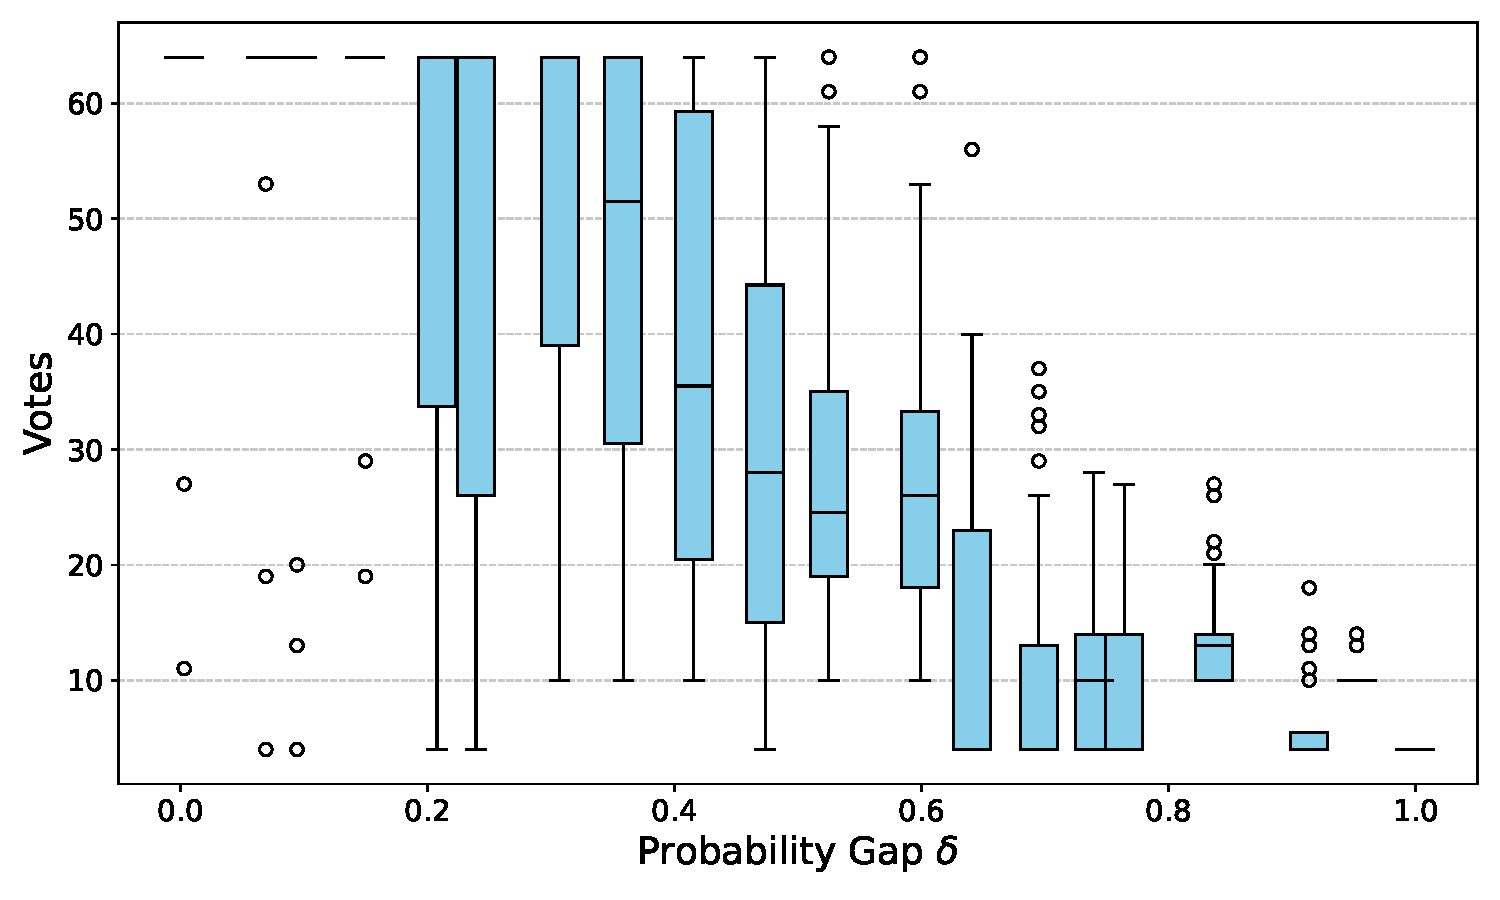
\includegraphics[width=\textwidth]{figs/truncated_beta_prior_stopping_5.pdf}
      \caption{Truncated Beta prior (A).}
      \label{fig:votes_truncated_beta_prior}
  \end{subfigure}
  \hfill
  \begin{subfigure}{0.49\textwidth}
      \centering
      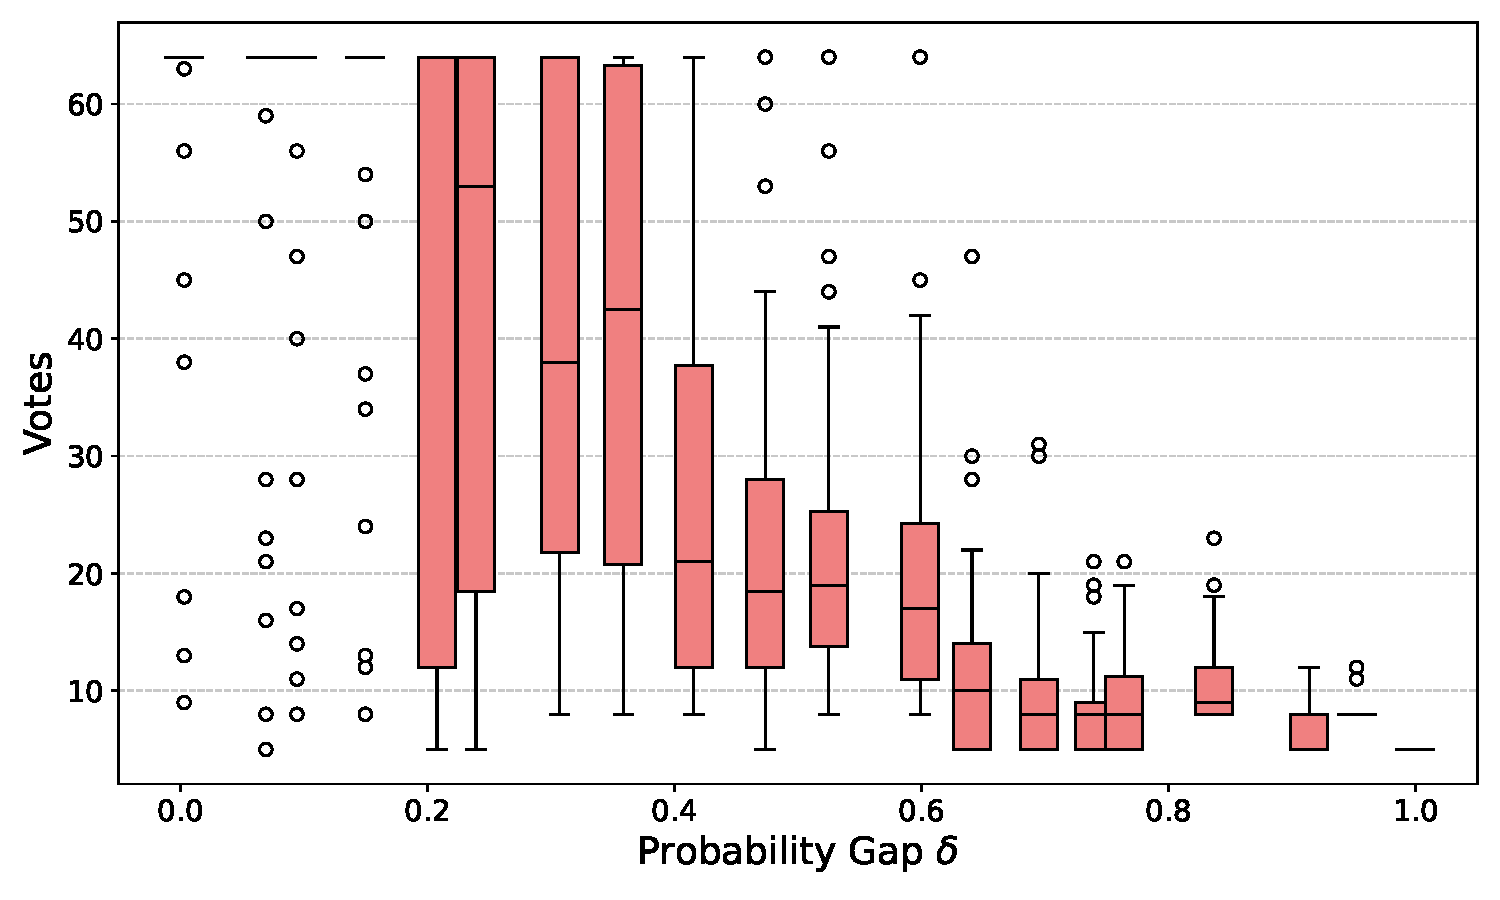
\includegraphics[width=\textwidth]{figs/delta_dirac_prior_stopping_5.pdf}
        \caption{Updating point prior (B.1).}
      \label{fig:votes_delta_dirac_prior}
  \end{subfigure}
  \vfill
  \vspace{8pt}
    \begin{subfigure}{0.49\textwidth}
      \centering
      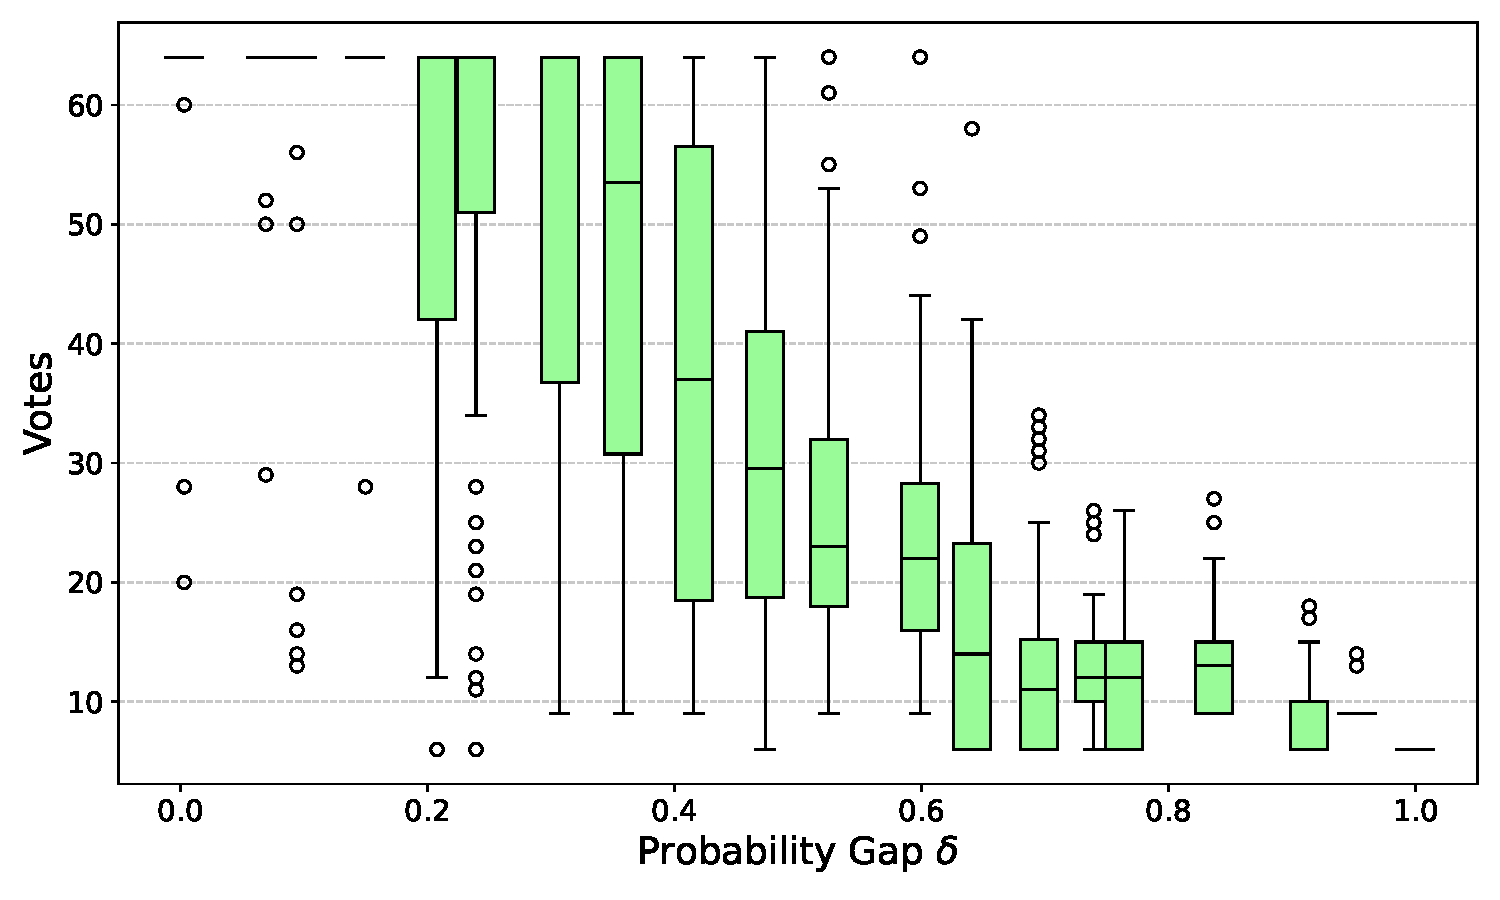
\includegraphics[width=\textwidth]{figs/updating_point_prior_ratio_stopping_5.pdf}
        \caption{Updating point prior (B.2).}
      \label{fig:votes_delta_dirac_prior_ratio_updates}
  \end{subfigure}
  \caption{Boxplots showing the distribution of the number of votes required until stopping under the MMC rule as a function of the probability gap $\delta = p_{c^\star}- p_{j^\star}$. Results are shown for $\varepsilon = 0.1$ with a maximum budget of 64 votes.}
  \label{fig:synthetic_data_stopping_rule}
\end{figure}
